\section{LiTFSI in water}

In search for new electrolytes, superconcentrated solutions of salts in water, called "water-in-salt" electrolytes, have recently attracted significant attention~\cite{li-tfsi-h2o-2,li-tfsi-h2o-3,li-tfsi-h2o-4,li-tfsi-h2o-5,li-tfsi-h2o-6,li-tfsi-h2o-7}. An example of such a~system are LiTFSI solutions in water, in which concentrations up to 21m can be achieved. Measured IR spectra show clear dependence on salt content~\cite{li-tfsi-h2o-1}.

In this section results for systems consisting of LiTFSI in water in different concentration are presented. As this is the subject of a~recent study, at the moment of writing this thesis they are not published in any journal yet.

\begin{table}[ht]
  \centering
  \caption{Compositions of LiTFSI/H$_2$O systems}
  \label{tab:li-tfsi-h2o-compositions}
\begin{tabular}{ccc}
\toprule
system & LiTFSI & H2O \\
\midrule
1m     & 4      & 222 \\
5m     & 15     & 167 \\
10m    & 22     & 122 \\
20m    & 30     & 83  \\
\bottomrule
\end{tabular}
\end{table}

Four systems with different concentration of lithium salt were studied by AIMD: 1m, 5m, 10m and 20m. Their compositions are listed in Table~\ref{tab:li-tfsi-h2o-compositions}. For every system two independent simulations with different initial structures were performed and for each of them 40~ps of trajectory was collected, and the last 30~ps was used for analysis. Time step of~1.0~fs was used.

\begin{figure}[ht]
    \centering
    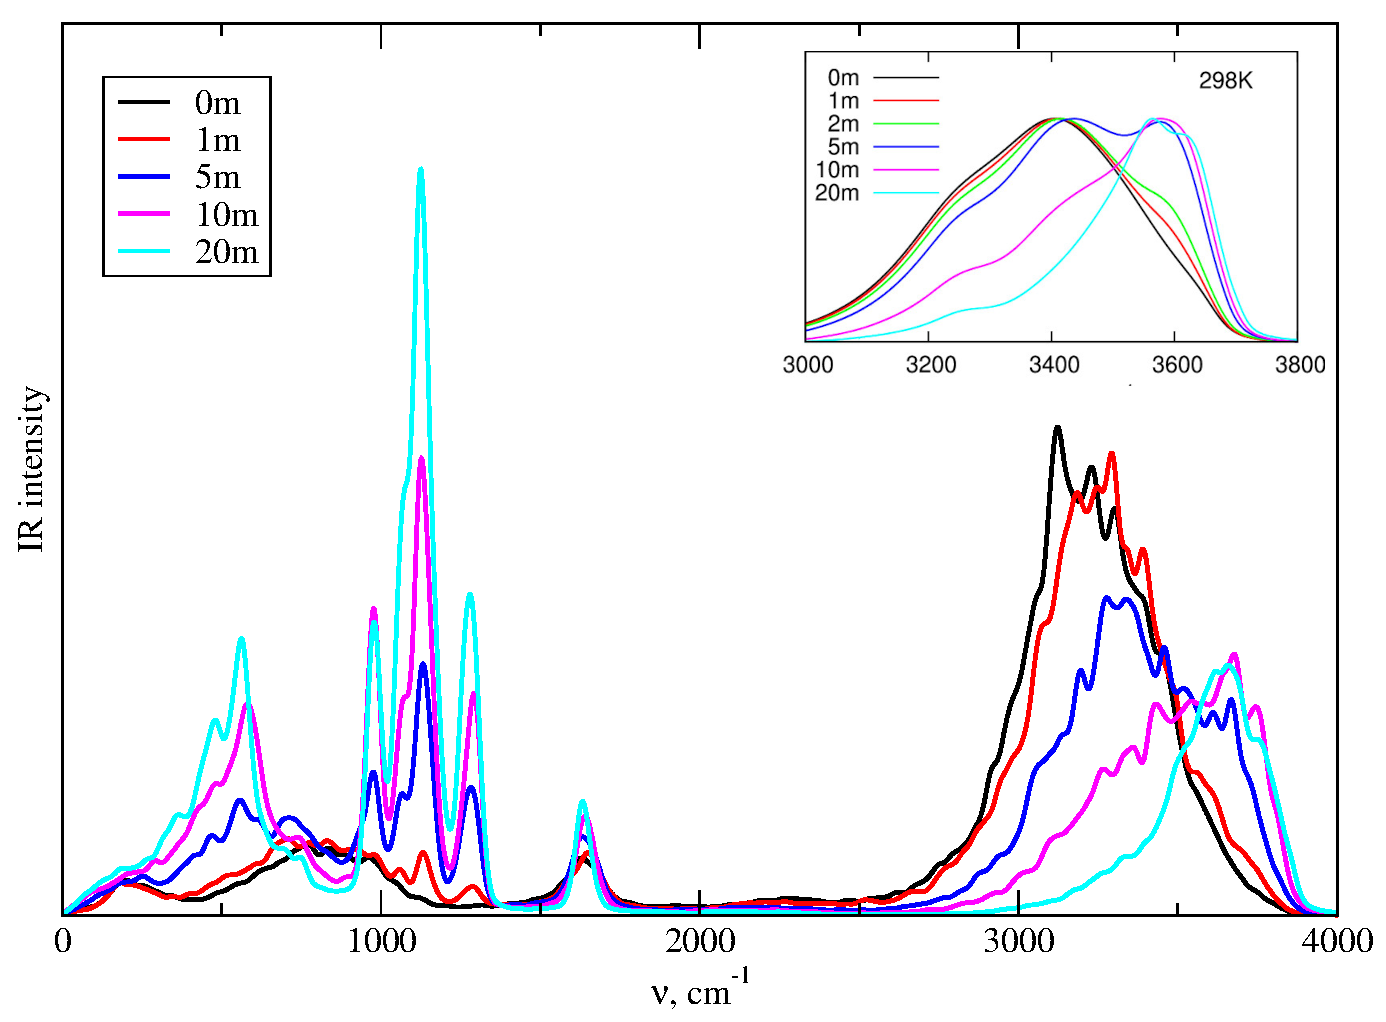
\includegraphics[width=0.7\textwidth]{img/4-ir-spectra-from-aimd-simulations/5-li-tfsi-h2o/averages-with-water.png}
    \caption{Infrared spectra obtained from AIMD for LiTFSI in H$_2$O systems, inset contains experimental spectra in the range of O-H vibrations from~\cite{li-tfsi-h2o-1}}
    \label{fig:li-tfsi-h2o-ir-averages}
\end{figure}

Figure~\ref{fig:li-tfsi-h2o-ir-averages} presents IR spectra averaged over replicas for each studied system. Below 2000~cm$^{-1}$ for every system there is a~visible band at about 1650~cm$^{-1}$ which was present at neat water spectrum presented in Figure~\ref{fig:il-h2o-ir-spectra}. Bands below this frequency have growing intensity with growing concentration of lithium salt, for the most diluted system they are quite indistinct. Their shape is similar as for the prevoius system and they could be related to vibrations in TFSI$^{-}$ anion, the growing intensity is the effect of increase of salt concentration in the system.

Above 3000~cm$^{-1}$ the position of the band, which may be related to O-H vibration in water molecule, is systematically shifted to higher frequencies with growing concentration of the salt, with the maximum moving from about 3150~cm$^{-1}$ to about 3650~cm$^{-1}$. It is similar to the effect observed for EMIM-TFSI with water mixtures and may be attributed to changing environment of hydrogen bonds. For the most diluted system, the most of HBs are formed between water molecules, due to low amount of salt, thus the maximum of the O-H band is the lowest among considered systems. With increasing salt amount, the water-water HBs are gradually replaced with water-TFSI$^{-}$ HBs what changes the frequency to higher values. The observed tendency stands in an agreement with experimental results, however the maximum of the peak for bulk water and diluted solutions in AIMD spectra are shifted towards lower frequencies. For further research it is planned to analyse the local environment of water molecules in these systems, in particular to calculate average number of water-water and water-TFSI$^{-}$ hydrogen bonds and to correlate it to the frequency of O-H vibrations.